% Created 2024-12-05 Do 18:46
% Intended LaTeX compiler: lualatex
\documentclass{mimosis}
                  \usepackage[hyperref,x11names]{xcolor}
\usepackage[
colorlinks = true,
citecolor  = RoyalBlue,
linkcolor  = RoyalBlue,
urlcolor   = RoyalBlue,
unicode
]{hyperref}
\usepackage{fontspec}
\usepackage{ltablex}
\usepackage{unicode-math}
\setmonofont{DejaVu Sans Mono}[Scale=0.8]
\newenvironment{abstract} {}{}
\usepackage{abstract}

%% ox-latex features:
%   !announce-start, bibliography-biblatex, !guess-pollyglossia, !guess-babel,
%   !guess-inputenc, caption, image, bibliography-biblatex-resources,
%   !announce-end.

\usepackage{biblatex}


\usepackage{capt-of}

\usepackage{graphicx}

\addbibresource{~/org/resources/bibliography/refs.bib}

%% end ox-latex features

\author{ProceduralTree}
\date{\today}
\title{Project Thesis}
\hypersetup{
 pdfauthor={ProceduralTree},
 pdftitle={Project Thesis},
 pdfkeywords={},
 pdfsubject={},
 pdfcreator={Emacs 29.4 (Org mode 9.8-pre)}, 
 pdflang={English}}
\begin{document}

\maketitle
\setcounter{tocdepth}{1}
\tableofcontents

\begin{abstract}
This work shows sensitivity of boundary conditions for two different finite difference approaches to solving the Cahn-Hilliard equation
\end{abstract}
\chapter{Introduction}
\label{sec:org86eb858}
This project thesis builds upon the work in our bachelor thesis, by introducing a simple boundary condition approach to a variation of the solver used therein. In Chapter \ref{sec:orga3eaff8} we introduce the Cahn-Hilliard Equation in the formulation that we use for this project. This project used a two-dimensional second order version of this CH equation rather than the usual 1D 4th order one, to simplify the numerical implementation. The solver itself builds upon a finite difference discretization of this equation. In Chapter \ref{sec:org60b5500}, together with the discrete domains, on which we run our numerical solver, we introduce a Jacoby iteration to solve the linear system derived from the aforementioned discretization.  The numerical solver in this thesis is GPU accelerated, and the discretization we chose to base our solver on is capable to calculate on all domains as long as a characteristic function is given. Therefore, we introduce two domains, on which we present our findings. The primary goal of this work is then the boundary condition approach in Chapter \ref{sec:org0a373e8}. Conceptionally the boundary condition we introduce simply consists of a constant value added in the linear system to all equations corresponding to grid cells on the boundary. The actual implementation is capable of doing this for arbitrary domains. We present the results of this method on two Domains, a square one in \ref{sec:orgb19866a} and a circular domain in \ref{sec:org0841c9c}
\chapter{Fundamentals}
\label{sec:orga3eaff8}
The Cahn-Hilliard (CH) equation is a diffuse interface coupling equation used for interpolating between different approach in different formulas. We use it in the following form:
\begin{equation}
\begin{aligned}
\partial_{t}\phi(x,t) &=  \nabla \cdot(M(\phi)\nabla\mu) \\
\mu &= - \varepsilon^2 \Delta\phi  + W'(\phi)
\end{aligned}
\end{equation}
Furthermore our solver implements the ansatz proposed by the autors\autocite{SHIN20117441}.
\begin{equation}
\label{eq:ansatz}
\begin{aligned}
\frac{\phi_{ij}^{n+1} - \phi_{ij}^n}{\Delta t}  &=  \nabla _d \cdot (G_{ij} \nabla_d \mu_{ij}^{n+\frac{1}{2}} )  \\
 \mu_{ij}^{n+\frac{1}{2}} &= 2\phi_{ij}^{n+1} - \varepsilon^2  \nabla_d \cdot  (G_{ij} \nabla _d \phi_{ij}^{n+1} ) + W'(\phi_{ij}^n) - 2\phi _{ij}^n
\end{aligned}
\end{equation}
Although we use as slightly different implementation as in the bachelor thesis\autocite{Ulmer_CHRelaxed_2024}.,  use the same discretizations and notation.

\begin{center}
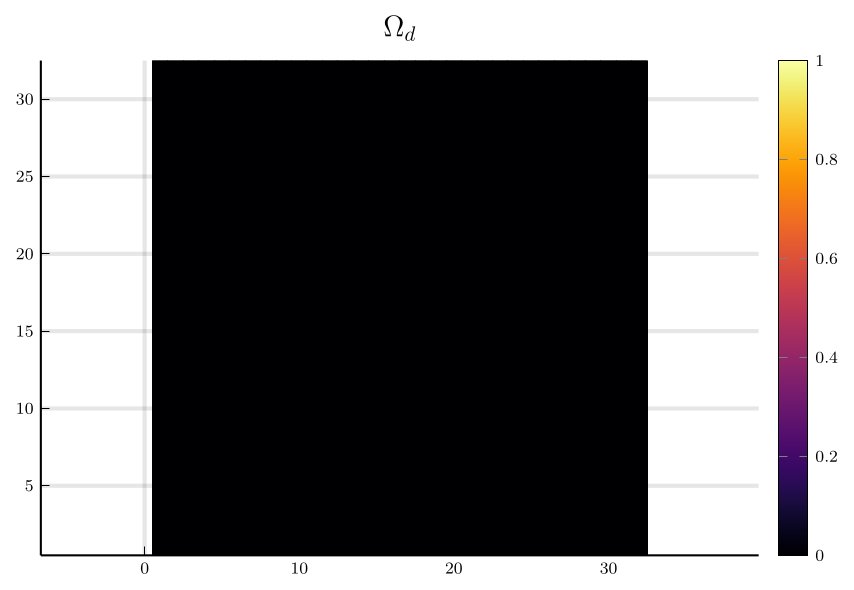
\includegraphics[width=.9\linewidth]{images/domain.png}
\label{}
\end{center}
\section{Notation}
\label{sec:org6a9a752}
We use the following differential quotients:
\begin{align}
D_xf_{i+\frac{1}{2} j} &= \frac{f_{i+1j} - f_{ij}}{h} & D_yf_{ij+\frac{1}{2}} &= \frac{f_{ij+1} - f_{ij}}{h}
\end{align}
and define a discrete gradient as.
\begin{equation}
\nabla_d f_{ij} = (D_x f_{i+1j} , \ D_y f_{ij+1})
\end{equation}
see\autocite{Ulmer_CHRelaxed_2024}
\chapter{Boundary adaptation}
\label{sec:org0a373e8}
The solver we use as reference guaranties no flux boundary conditions at a discrete level by setting \(\nabla \phi_{ij} = 0\) for \(\phi_{ij} \in \partial \Omega_{d}\) this is done by multiplying with the Characteristic function of \(\Omega_{d}\)
\begin{equation}
G_{ij}=
\begin{cases}
1 \,, x_{ij} \in \Omega \\
0 \,, x_{ij} \not\in \Omega \\
\end{cases}
\end{equation}
To accommodate different boundary conditions, we bias \(\nabla_d \cdot (G_{ij} \nabla_d \phi_{ij})\) in grid points next to the boundary. We determine those points using a centered difference scheme on \(G\)
\begin{equation}
B_{ij} = \max\left(  |G_{i+\frac{1}{2}j} - G_{i-\frac{1}{2}j}| , |G_{ij+\frac{1}{2}} - G_{ij-\frac{1}{2}}|\right) * C
\end{equation}
Where \(C\) is a constant we chose freely. For example on a 32x32 Domain with \(C=1\) the Boundary fiels \(\mathbf{B}\) appears as follows


\begin{figure}[htbp]
\centering
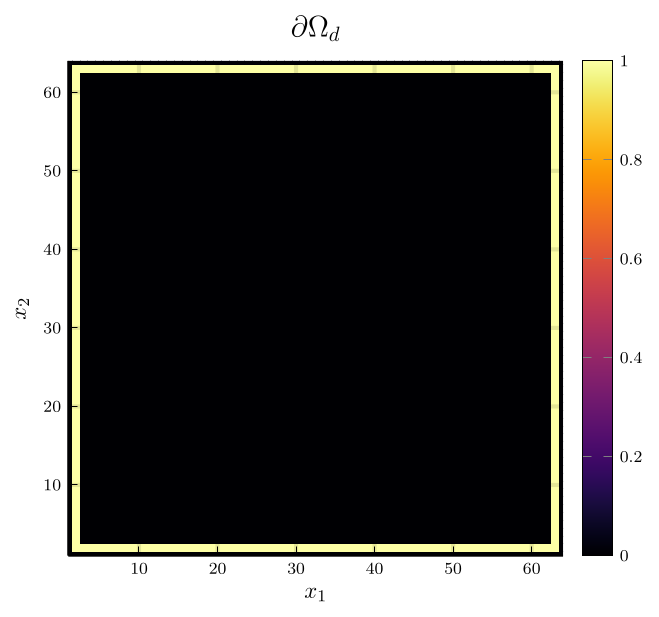
\includegraphics[width=.9\linewidth]{images/boundary.png}
\caption{\label{fig:boundary-square}visualization of all grid-cells adjacent to the boundary \(\partial \Omega_{d}\) of a square domain}
\end{figure}




\begin{figure}[htbp]
\centering
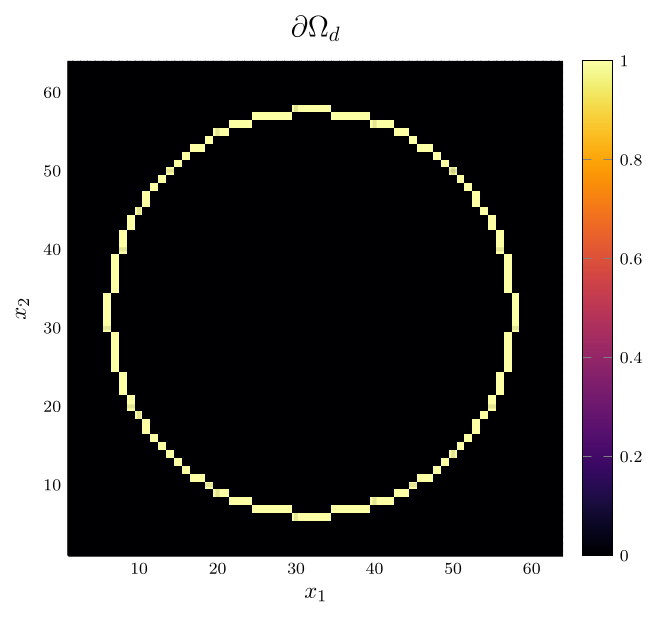
\includegraphics[width=.9\linewidth]{images/boundary-circle.png}
\caption{\label{fig:boundary-circle}visualization of all grid-cells adjacent to the boundary \(\partial \Omega_{d}\) of a circular domain}
\end{figure}



We then state the adapted approach as :
\begin{equation}
\label{eq:second-order-adapted-ansatz}
\begin{aligned}
\frac{\phi_{ij}^{n+1} - \phi_{ij}n}{\Delta t}  &=  \nabla _d \cdot (G_{ij} \nabla_d \mu_{ij}^{n+\frac{1}{2}} )  \\
 \mu_{ij}^{n+\frac{1}{2}} &= 2\phi_{ij}^{n+1} - \varepsilon^2  \nabla_d \cdot  (G_{ij} \nabla _d \phi_{ij}^{n+1} ) + B_{ij} + W'(\phi_{ij}^n) - 2\phi _{ij}^n
\end{aligned}
\end{equation}
\chapter{Numerical solver}
\label{sec:org60b5500}
contrary to the solver proposed in\autocite{Ulmer_CHRelaxed_2024} we do not use a multi-grid Gauss-Seidel Solver to solve the linear system, and use a Jacoby solver instead, since it is easier to parrallize.
Similar to \autocite{Ulmer_CHRelaxed_2024} we linearise \eqref{eq:second-order-adapted-ansatz} to
\begin{equation}
\begin{aligned}
\frac{\phi_{ij}^{n+1}}{\Delta t}  -  \nabla _d \cdot (G_{ij} \nabla_d \mu_{ij}^{n+\frac{1}{2}} ) &= \frac{ \phi_{ij}^n}{\Delta t}  \\
 \mu_{ij}^{n+\frac{1}{2}} - 2\phi_{ij}^{n+1} + \varepsilon^2  \nabla_d \cdot  (G_{ij} \nabla _d \phi_{ij}^{n+1} ) + B_{ij} &=2\phi _{ij}^n - W'(\phi_{ij}^n)
\end{aligned}
\end{equation}
after some rearranging we note, that the left hand side is linear and, the right hand side is solely dependent on the previous time step. Therefore this constitutes a linear system, wich we solve with a Jacoby method, the element wise formula of wich is given as follows:
Provided the \(mth\) Jacoby iteration has been computed, the \(m+1th\) iteration is computed by solving
\begin{equation}
\begin{aligned}
\frac{\phi_{ij}^{n+1,m+1}}{\Delta t}  -  \nabla _d \cdot (G_{ij} \nabla_d \mu_{ij}^{n+\frac{1}{2},m+\frac{1}{2}} ) &= \frac{ \phi_{ij}^{n}}{\Delta t}  \\
 \mu_{ij}^{n+\frac{1}{2},m} - 2\phi_{ij}^{n+1,m} + \varepsilon^2  \nabla_d \cdot  (G_{ij} \nabla _d \phi_{ij}^{n+1,m+\frac{1}{2}} ) + B_{ij} &=2\phi _{ij}^n - W'(\phi_{ij}^n)
\end{aligned}
\end{equation}
for \(\phi_{ij}^{n+1,m+1} , \mu_{ij}^{n+\frac{1}{2},m+1}\),
where \(\nabla _d \cdot (G_{ij} \nabla_d \mu_{ij}^{n+\frac{1}{2},m+\frac{1}{2}} )\) and \(\nabla_d \cdot  (G_{ij} \nabla _d \phi_{ij}^{n+1,m+\frac{1}{2}} )\).  Use the results from the previous jacoby step for values off the center. eg.
\begin{equation}
\begin{aligned}
 \nabla _d \cdot (G_{ij} \nabla_d \phi_{ij}^{n+1,m+\frac{1}{2}} )  =&
\frac{1}{h^2} (
G_{i+\frac{1}{2}j}\phi_{i+1j}^{n+1,m}
+ G_{i-\frac{1}{2}j}\phi_{i-1j}^{n+1,m} \\
& + \quad G_{ij+\frac{1}{2}}\phi_{ij+1}^{n+1,m}
+ G_{ij-\frac{1}{2}}\phi_{ij-1}^{n+1,m}
 ) \\
& -
\left(
 G_{i+\frac{1}{2}j}
 + G_{i-\frac{1}{2}j}
 + G_{ij+\frac{1}{2}}
 + G_{ij-\frac{1}{2}}
\right)\phi_{ij}^{n+1,m+1}
\end{aligned}
\end{equation}
our implementation makes use of julia to dispatch the solution for each element in paralell on the GPU. The full implementation of the jacoby iteration is given as:
\begin{verbatim}
@kernel function jacoby!(
    Φ,
    M,
    @Const(Ξ),
    @Const(Ψ),
    @Const(h),
    @Const(ε),
    @Const(Δt),
    @Const(iterations)
)
    I   = @index(Global, Cartesian)
    Id  = oneunit(I)
    Ids = CartesianIndices(M)
    Ix = CartesianIndex(1, 0)
    Iy = CartesianIndex(0, 1)
    if I in (Ids[begin]+Id:Ids[end]-Id)
        g = G(2 * I + Ix, Ids) + G(2 * I + Iy, Ids) + G(2 * I - Ix, Ids) + G(2 * I - Iy, Ids)
        a1 = 1/Δt
        a2 = -1* ε^2/h^2 * g  - 2
        b1 = 1/h^2 * g
        b2 = 1
        for _ = 1:iterations

            Σμ = G(2 * I + Ix, Ids) * M[I+Ix] + G(2 * I + Iy, Ids) * M[I+Iy] + G(2 * I - Ix, Ids) * M[I-Ix] + G(2 * I - Iy, Ids) * M[I-Iy]

            Σϕ = G(2 * I + Ix, Ids) * Φ[I+Ix] + G(2 * I + Iy, Ids) * Φ[I+Iy] +G(2 * I - Ix, Ids) * Φ[I-Ix] +G(2 * I - Iy, Ids) * Φ[I-Iy]

            c1 = Ξ[I] + 1/h^2   * Σμ
            c2 = Ψ[I] - ε^2/h^2 * Σϕ

            # stupid matrix solve
            @inline Φ[I] = (c1*b2 - c2*b1) / (a1*b2 - a2*b1)
            @inline M[I] = (a1*c2 - a2*c1) / (a1*b2 - a2*b1)
            #
            @synchronize()
        end

    end
end
\end{verbatim}
\chapter{Numerical evaluation}
\label{sec:orgb19866a}
\section{Experiments}
\label{sec:orgcc83298}
To begin our evaluations we tested constant values for \(B_{ij}\) on the boundary.
Initially we tested setting \(C=0\) as it is equivalent to the no-flux boundary condition of the unmodified solver. For \(C = 0\) ,as seen in \ref{fig:angle0} the interface lies orthogonal on the boundary as expected for a CH solver with no-flux boundary conditions.
For \(B_{ij} \in \{-1,1\}\) we observed behaviour expected of hydrophobic / hydrophilic substances on the boundary, where \(B_{ij}=1\) resulted in the one phase pearling of the boundary, while the other semed attracted. this manifested on apparent contact angles of 180° and 0° respectivly. Using \(B_{ij} = -1\) results in the opposite behavior.


\begin{figure}[htbp]
\centering
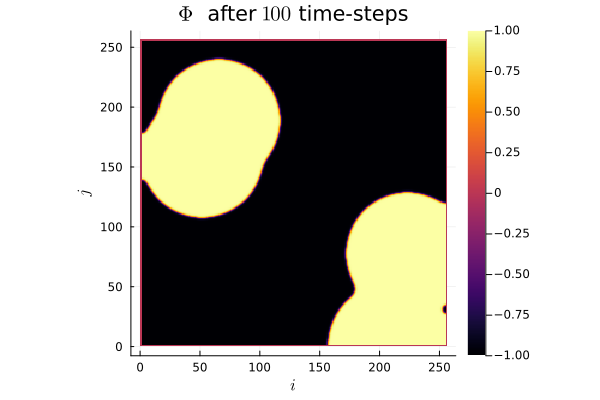
\includegraphics[width=.9\linewidth]{images/baseline.png}
\caption{\label{fig:angle0}phase-field \(\phi\) after 100 time-steps with \(C=0\) emmulating no-flux boundary.}
\end{figure}

To showcase the relative stability, and the effect off the constant boundary proposed in TODO we evaluate our solver with different constant values \(C\). In \ref{fig:angle1} we employ a constant value of \(C=1\) and observe the phase corresponding to \(\phi = 1\) puling away from the boundary. the contact angle between phase 1 and the boundary approaches 180° ie. the interface runs parallel to the boundary.
\begin{center}
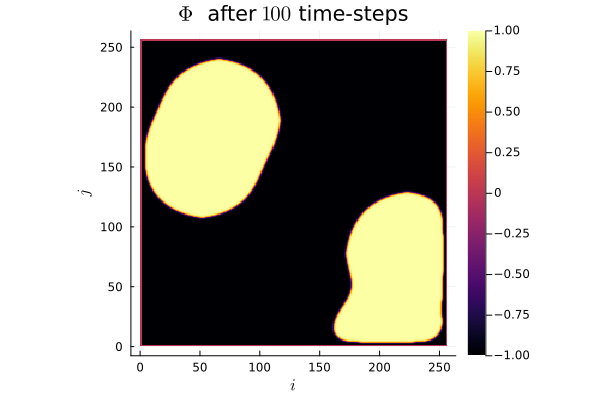
\includegraphics[width=.9\linewidth]{images/angle1.png}
\label{fig:angle1}
\end{center}


In \ref{fig:angle-1} we try the opposite as bevore. And we obsesrve corresponding behaviour. When using a value of \(C=-1\) we observe behaviour opposite to before. Where the contact angle on the boundary lies at 0°, the interface runs parallel to the boundary again.
\begin{figure}[htbp]
\centering
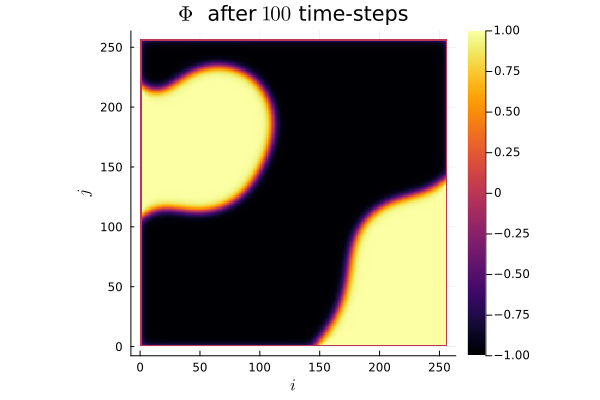
\includegraphics[width=.9\linewidth]{images/angle-.png}
\caption{\label{fig:angle-1}phase-field \(\phi\) after 100 time-steps with \(C=-1\)}
\end{figure}

we observe the most interessting behaviour for values between \((-1,1)\), where we observe the contact angle of the interafce on the boundary to change from parallel 0° to parallel 180°.
\begin{verbatim}
include("src/solvers.jl")
θ = -5f-1
n = 100
arr = _init()
d = domain(get_backend(arr) , 256 , size(arr))
d(arr)
h = 25e-5
solution = solve(arr , n , θ=θ)
h1 = heatmap(Array(solution) , aspect_ratio=:equal , clims=(-1,1), lims=(0,size(solution,1)), widen=1.06 , title=L"h=%$h")
h = 20e-5
solution = solve(arr , n , θ=θ)
h2 = heatmap(Array(solution) , aspect_ratio=:equal , clims=(-1,1), lims=(0,size(solution,1)), widen=1.06 , title=L"h=%$h")
h = 15e-5
solution = solve(arr , n , θ=θ)
h3 = heatmap(Array(solution) , aspect_ratio=:equal , clims=(-1,1), lims=(0,size(solution,1)), widen=1.06 , title=L"h=%$h")
h = 10e-5
solution = solve(arr , n , θ=θ)
h4 = heatmap(Array(solution) , aspect_ratio=:equal , clims=(-1,1), lims=(0,size(solution,1)), widen=1.06 , title=L"h=%$h")
plot(h1,h2,h3,h4)
\end{verbatim}

\begin{center}
\includegraphics[width=.9\linewidth]{/tmp/babel-frcHT2/julia-LrFbWa.png}
\label{fig:random-square}
\end{center}

\phantomsection
\label{}
\begin{verbatim}
Plots.AnimatedGif("/home/proceduraltree/Projects/JuliaGPUTest/animations/h.mp4")
\end{verbatim}


\phantomsection
\label{}
\begin{verbatim}
Plots.AnimatedGif("/home/proceduraltree/Projects/JuliaGPUTest/animations/epsilon.mp4")
\end{verbatim}
\chapter{Numerical evaluation on a circle}
\label{sec:org0841c9c}
\section{Experiments}
\label{sec:org5591fd6}
The original solver presented in\autocite{SHIN20117441}  was able to solve the CH equation on arbitrary domains. Since the addition of our boundary function depends soley on the characteristic function of the discrete domain, we are able to use our approach on diferent Domains, by providing a different characteristic function. We present the results of which in this chapter.
To show the behavior of the CH sover in \ref{fig:angle0c}, we first emplay no-flux boundary conditioons on a circular domain. We observe the interface perpendicular on the boundary, as we expect.

\phantomsection
\label{}
\begin{verbatim}
W′ (generic function with 1 method)
\end{verbatim}



\begin{figure}[htbp]
\centering
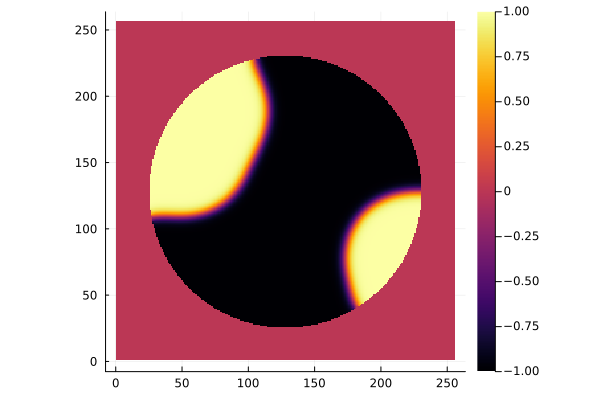
\includegraphics[width=.9\linewidth]{images/angle0c.png}
\caption{\label{fig:angle0c}\(\phi\) after 100 time steps on a circular domain with no-flux boundary-conditions after 100 time steps on a circular domain with no-flux}
\end{figure}



The results we oserve in \ref{fig:angle1c} are similar to the reults on a square domain in \ref{fig:angle1}. The contact angle is 18° i.e. the interface does not touch the boundary and runs parallel to it.
\begin{figure}[htbp]
\centering
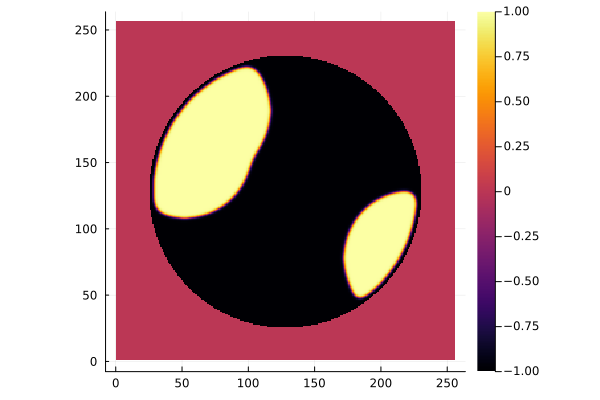
\includegraphics[width=.9\linewidth]{images/anfle1c.png}
\caption{\label{fig:angle1c}phase-field \(\phi\) after 100 time-steps with \(C=1\)}
\end{figure}

The results for \(C=-1\) in \ref{fig:angle-1c} on the circular domain, are similar to the results in \ref{fig:angle-1}  onth esqaure domain as well ,where the interface touches the boundary and iun parallel with a contact angle of 0°.
\begin{figure}[htbp]
\centering
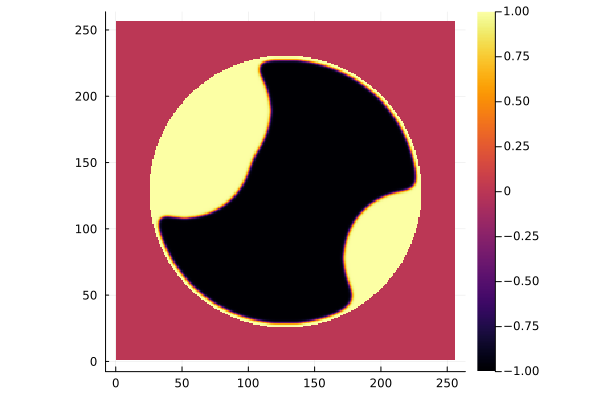
\includegraphics[width=.9\linewidth]{images/angle-1c.png}
\caption{\label{fig:angle-1c}phase-field \(\phi\) after 100 time-steps with \(C=-1\)}
\end{figure}


\begin{figure}[htbp]
\centering
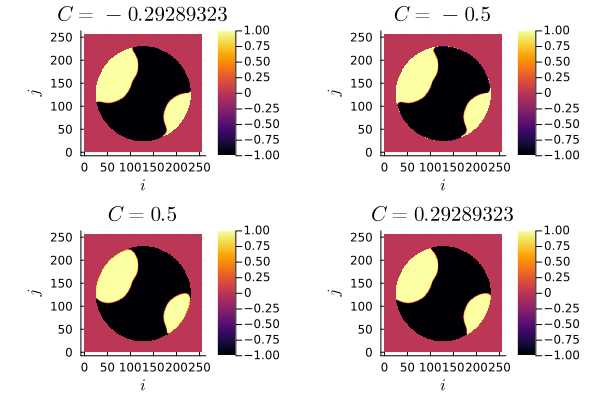
\includegraphics[width=.9\linewidth]{images/angle-multiplec.png}
\caption{\label{fig:angle-multiplec}phase-field \(\phi\) after 500 time-steps with \(C \in \{-1 + \frac{\sqrt{2}}{2} , -0.5 , 0.5 , 1 - \frac{\sqrt{2}}{2} \}\) on a circular domain.}
\end{figure}
\chapter{Relaxed}
\label{sec:orgae0d4d4}
\begin{center}
\includegraphics[width=.9\linewidth]{/tmp/babel-miHWkx/julia-h4yghb.png}
\label{}
\end{center}
\chapter{angle}
\label{sec:org470675e}
In previous experiments we noted the changing angle of the interface with changing input parameter. While we do not have a mathematical derrivation of this relation, we aim to provide numerical insight in this chapter. We calculate this angle as
\begin{align}
\label{eq:1}
\frac{\nabla_d \phi_{ij} \cdot \mathbf{n}}{\|\nabla_{d} \phi_{ij}\|} &= \cos(\theta)& & \phi_{ij} \in \partial\Omega_{d} = 0
\end{align}
for a single point P on the interface and near the boundary. Since we need a finite diference to evaluate \ref{eq:1}, we do not select a point directly on the boundary and since we need a point on the interface where \(\nabla \phi_{ij}\) is large, we select
\begin{equation}
\label{eq:2}
P = argmax \nabla \phi_{ij} \qquad \phi_{ij} \in \partial \Omega
\end{equation}
\begin{center}
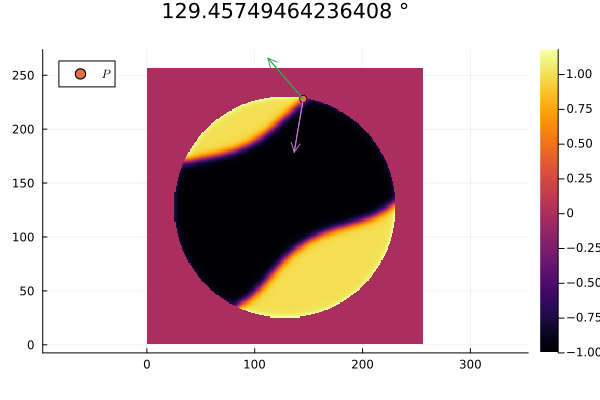
\includegraphics[width=.9\linewidth]{images/angle.png}
\label{}
\end{center}

\begin{longtable}{rr}
\caption{\label{angle-table}value for \(\theta\) and corresponding angle \(\alpha\) after 200 time-steps}
\\
-0.1 & 173.49096591056502\\
-0.095 & 173.10715739345923\\
-0.09 & 172.18364087939332\\
-0.085 & 171.54740091859054\\
-0.08 & 171.3054040677464\\
-0.075 & 171.1455632002332\\
-0.07 & 171.02869693204397\\
-0.065 & 170.3901810227686\\
-0.06 & 170.0449796355949\\
-0.055 & 173.27274052589075\\
-0.05 & 170.3373892767722\\
-0.045 & 168.11953739721892\\
-0.04 & 167.41386769034298\\
-0.035 & 166.62088559081457\\
-0.03 & 164.9014365935728\\
-0.025 & 162.8061312020723\\
-0.02 & 159.92337650959868\\
-0.015 & 155.82320048245077\\
-0.01 & 147.4707481361878\\
-0.005 & 129.77836444929315\\
0.0 & 91.28977210940522\\
0.005 & 47.27538237804684\\
0.01 & 26.60911004838421\\
0.015 & 6.306468865037136\\
0.02 & 11.495581754132852\\
0.025 & 8.059259459078769\\
0.03 & 2.997826637980469\\
0.035 & 2.442790881259583\\
0.04 & 2.314200756133827\\
0.045 & 1.883610279597664\\
0.05 & 1.3567468712125557\\
0.055 & 0.8024311153759808\\
0.06 & 0.5869880299417852\\
0.065 & 0.4356076759230446\\
0.07 & 0.32719257485287145\\
0.075 & 0.03099970458170946\\
0.08 & 0.37685133141547533\\
0.085 & 0.4151229191583983\\
0.09 & 0.7049376111739059\\
0.095 & 0.8671639875701463\\
0.1 & 1.0282690721714873\\
\end{longtable}
\chapter{Summary and outlook}
\label{sec:org47750d2}

\chapter{References}
\label{sec:org67bd0e9}
\printbibliography
\end{document}
